Sapata conjugada é uma estrutura de fundação que associa dois ou mais pilares, alinhados num mesmo bloco.

*Inserir figuras

A fim de se obter as coordenadas do centro de carga (CC) do sistema, coloca-se um ponto referencial no centro de carga de $P1$ e realiza-se o somatório de momentos na direção $x$ na Figura $x$, ou seja:
$$(P1+P2)\cdot x=P2\cdot d_1$$

Isolando-se $x$ [que nesse caso é o centro de carga (CC) do sistema], tem-se:
\begin{equation}x=\frac{P2\cdot d_1}{P1+P2}\end{equation}

Da mesma maneira para a direção $y$, tem-se:
$$(P1+P2)\cdot y=P2\cdot d_2$$

Isolando-se $y$:
\begin{equation}y=\frac{P2\cdot d_2}{P1+P2}\end{equation}

A área de sapata conjugada necessária é obtida a partir das cargas dos pilares e da tensão admissível do solo ou, ainda, pelo produto de seus lados:
\begin{equation}A=\frac{P1+P2}{\sigma_s}=a\cdot b\end{equation}

Pode-se classificar a sapata conjugada quanto ao posicionamento dos pilares:

\textbf{Próximos à divisa}:
\begin{itemize}
	\item Pilar mais leve fica mais próximo da divisa;
	\item Pilar mais pesado fica mais próximo da divisa;
\end{itemize}

\textbf{Afastados da divisa}:
\begin{itemize}
	\item Pilares com o mesmo carregamento;
	\item Pilares com carregamentos diferentes.
\end{itemize}

Para o \textbf{primeiro caso}, onde o pilar mais leve fica mais próxim da divisa, pode-se encontrar a coordenada $x_{CC}$ estabelecendo-se um ponto de referência $PR$ e fazendo a somatória dos momentos fletores em relação àquele ponto. Como segue:

*Inserir figura

$$x_{CC}=\frac{P1\cdot\displaystyle\frac{b_0}{2}+P2\cdot\left(d_1+\displaystyle\frac{b_0}{2}\right)}{P1+P2}$$

Para o \textbf{segundo caso}, onde o pilar mais pesado fica mais próximo da divisa, deve-se utilizar o Método do Trapézio para encontrar as dimensões do seguinte sistema:

*Inserir figura:

O Método do Trapézio é realizado da seguinte forma:
\begin{enumerate}
	\item Calcular o centro de carga;
	\item Adotar o valor de $y=x_{CC}$
		\begin{equation}x_{CC}=\frac{P1\cdot x_1+P2\cdot x_2}{P1+P2}=y\end{equation}
	\item Estimar o valor de $c$ em ($c<3\cdot y$)
	\item Calcular a área da base da sapata:
		$$A=\frac{P1+P2}{\sigma_s}$$
		\begin{equation}A=(a+b)\cdot \frac{c}{2}\end{equation}
	\item Calcular a parcela $(a+b)$:
		\begin{equation}(a+b)=\frac{2\cdot A}{c}\end{equation}
	\item Calcular o valor de $b$:
		$$y=\frac{c}{3}\cdot\left[\frac{(a+b)+b}{a+b}\right]$$
		\begin{equation}b=\left[\frac{3\cdot y}{c}\cdot(a+b)\right]-(a+b)\end{equation}
	
	Se $b<60\;cm$, retornar ao passo onde se estima o valor de $c$, diminuir o seu valor e recalcular $b$, passando pelos tópicos intermediários novamente.
	\item Calcular $a$:
		\begin{equation}a=\frac{2\cdot A}{c}-b\end{equation}
\end{enumerate}

\textbf{Exercício}: Calcular a sapata para os seguintes pilares com uma tensão admissível do solo ($\sigma_s$) de $0,3\;MPa$ e $P1=P2=3000\;kN$:
\begin{figure}[H]
	\begin{center}
	\caption{Sistema de pilares do problema proposto.}
    	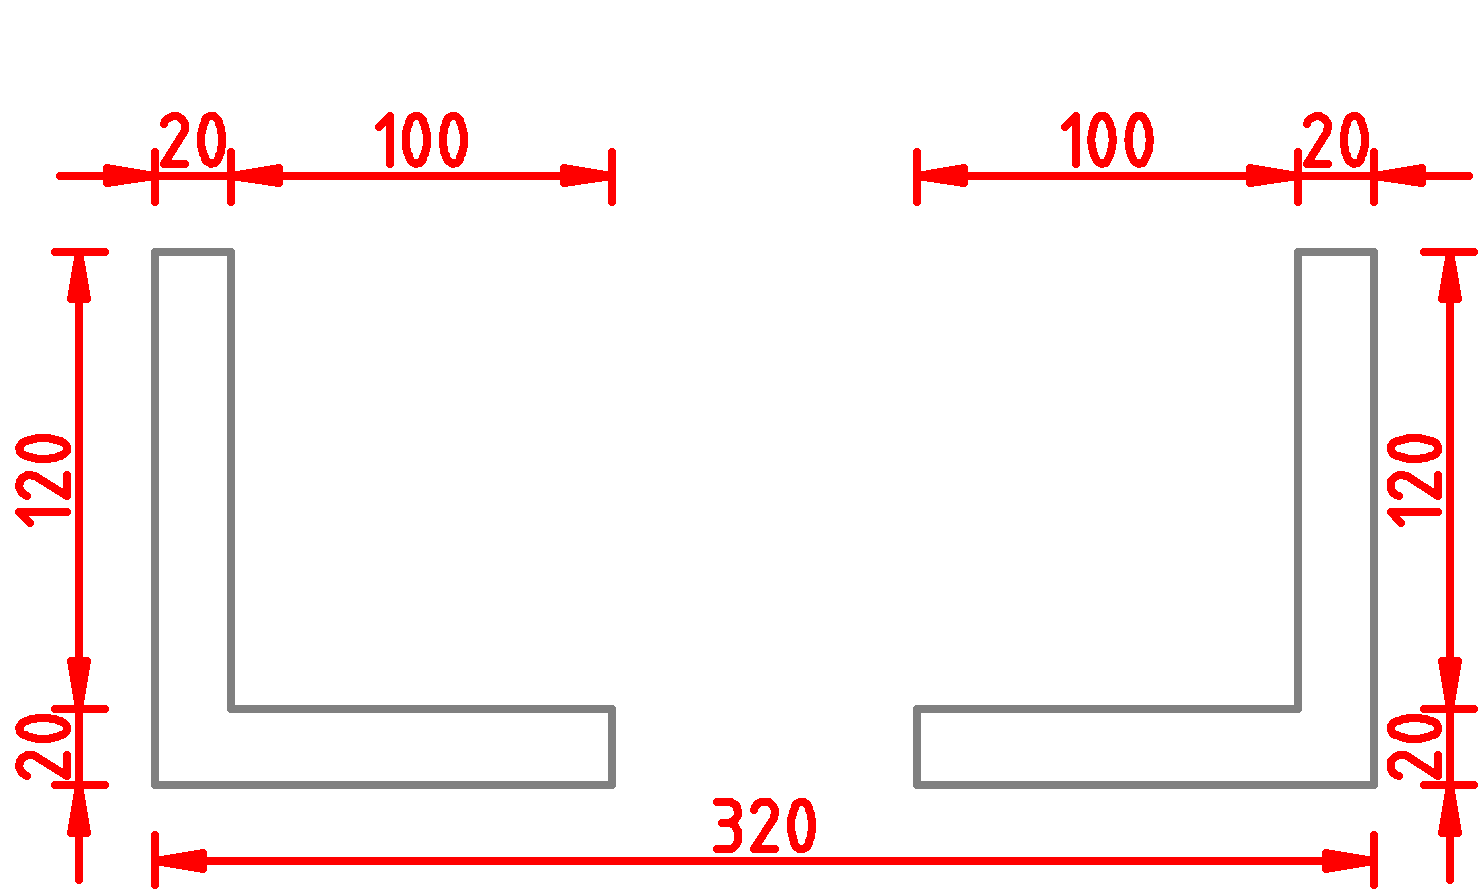
\includegraphics[width=0.7\textwidth]{Fundacoes-rasas-ou-diretas/Imagens/Exercicio-1-Sapata-conjugada.png}
	\end{center}
\end{figure}

O primeiro passo é \textbf{testar se a solução sapata isolada é possível de ser realizada}. Calcula-se, primeiramente, o CG de um dos pilares (sistema simétrico).
$$x_{CG}=\frac{(120\cdot20)\cdot10+(20\cdot120)\cdot60}{(120\cdot20)+(20\cdot120)}=35\;cm$$ 
$$y_{CG}=\frac{(120\cdot20)\cdot80+(20\cdot120)\cdot10}{(120\cdot20)+(20\cdot120)}=45\;cm$$
\begin{figure}[H]
	\begin{center}
	\caption{Centro de carga (CG) do pilar à esquerda.}
    	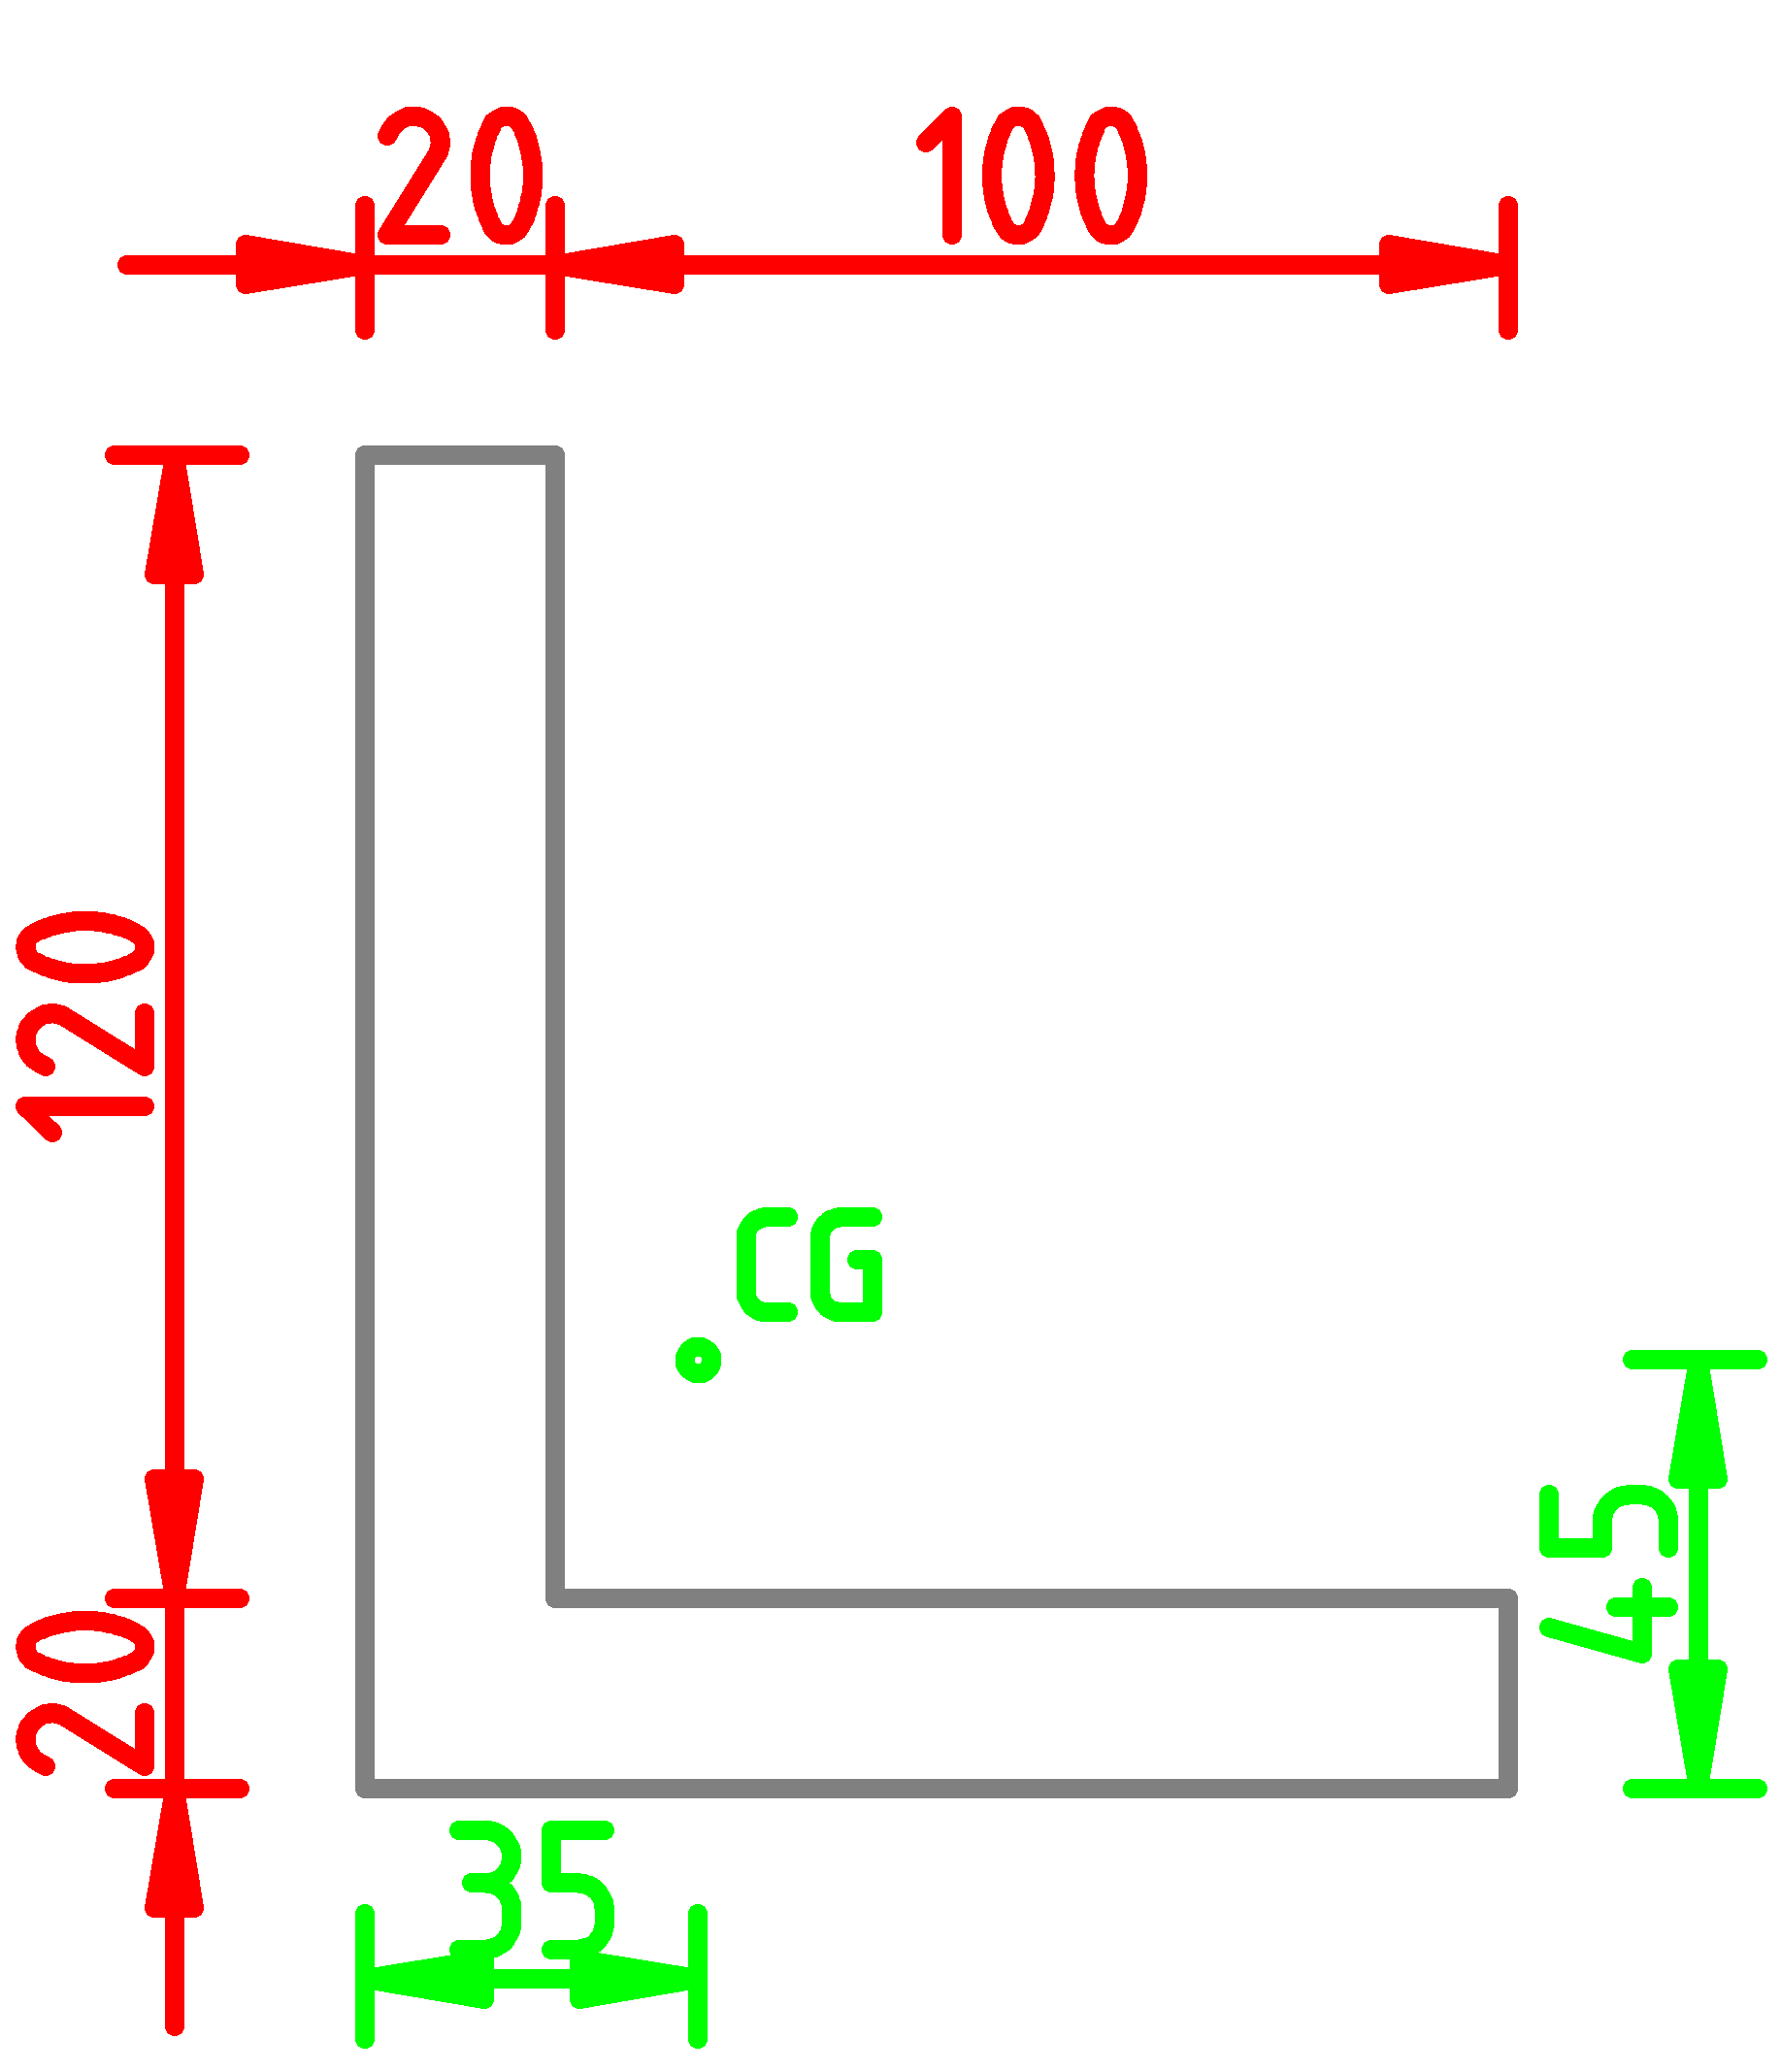
\includegraphics[width=0.4\textwidth]{Fundacoes-rasas-ou-diretas/Imagens/Exercicio-1-Sapata-conjugada-parte2.png}
	\end{center}
\end{figure}

Para encontrar $a_0$ e $b_0$ do pilar retangular equivalente, deve-se encontrar a maior distância do CG em ambos os eixos até as faces do pilar a partir do sistema de coordenadas adotado.
$$a_0=(140-45)\cdot2=190\;cm$$
$$b_0=(120-35)\cdot2=170\;cm$$
\begin{figure}[H]
	\begin{center}
	\caption{Pilar fictício para a sapata escolhida.}
    	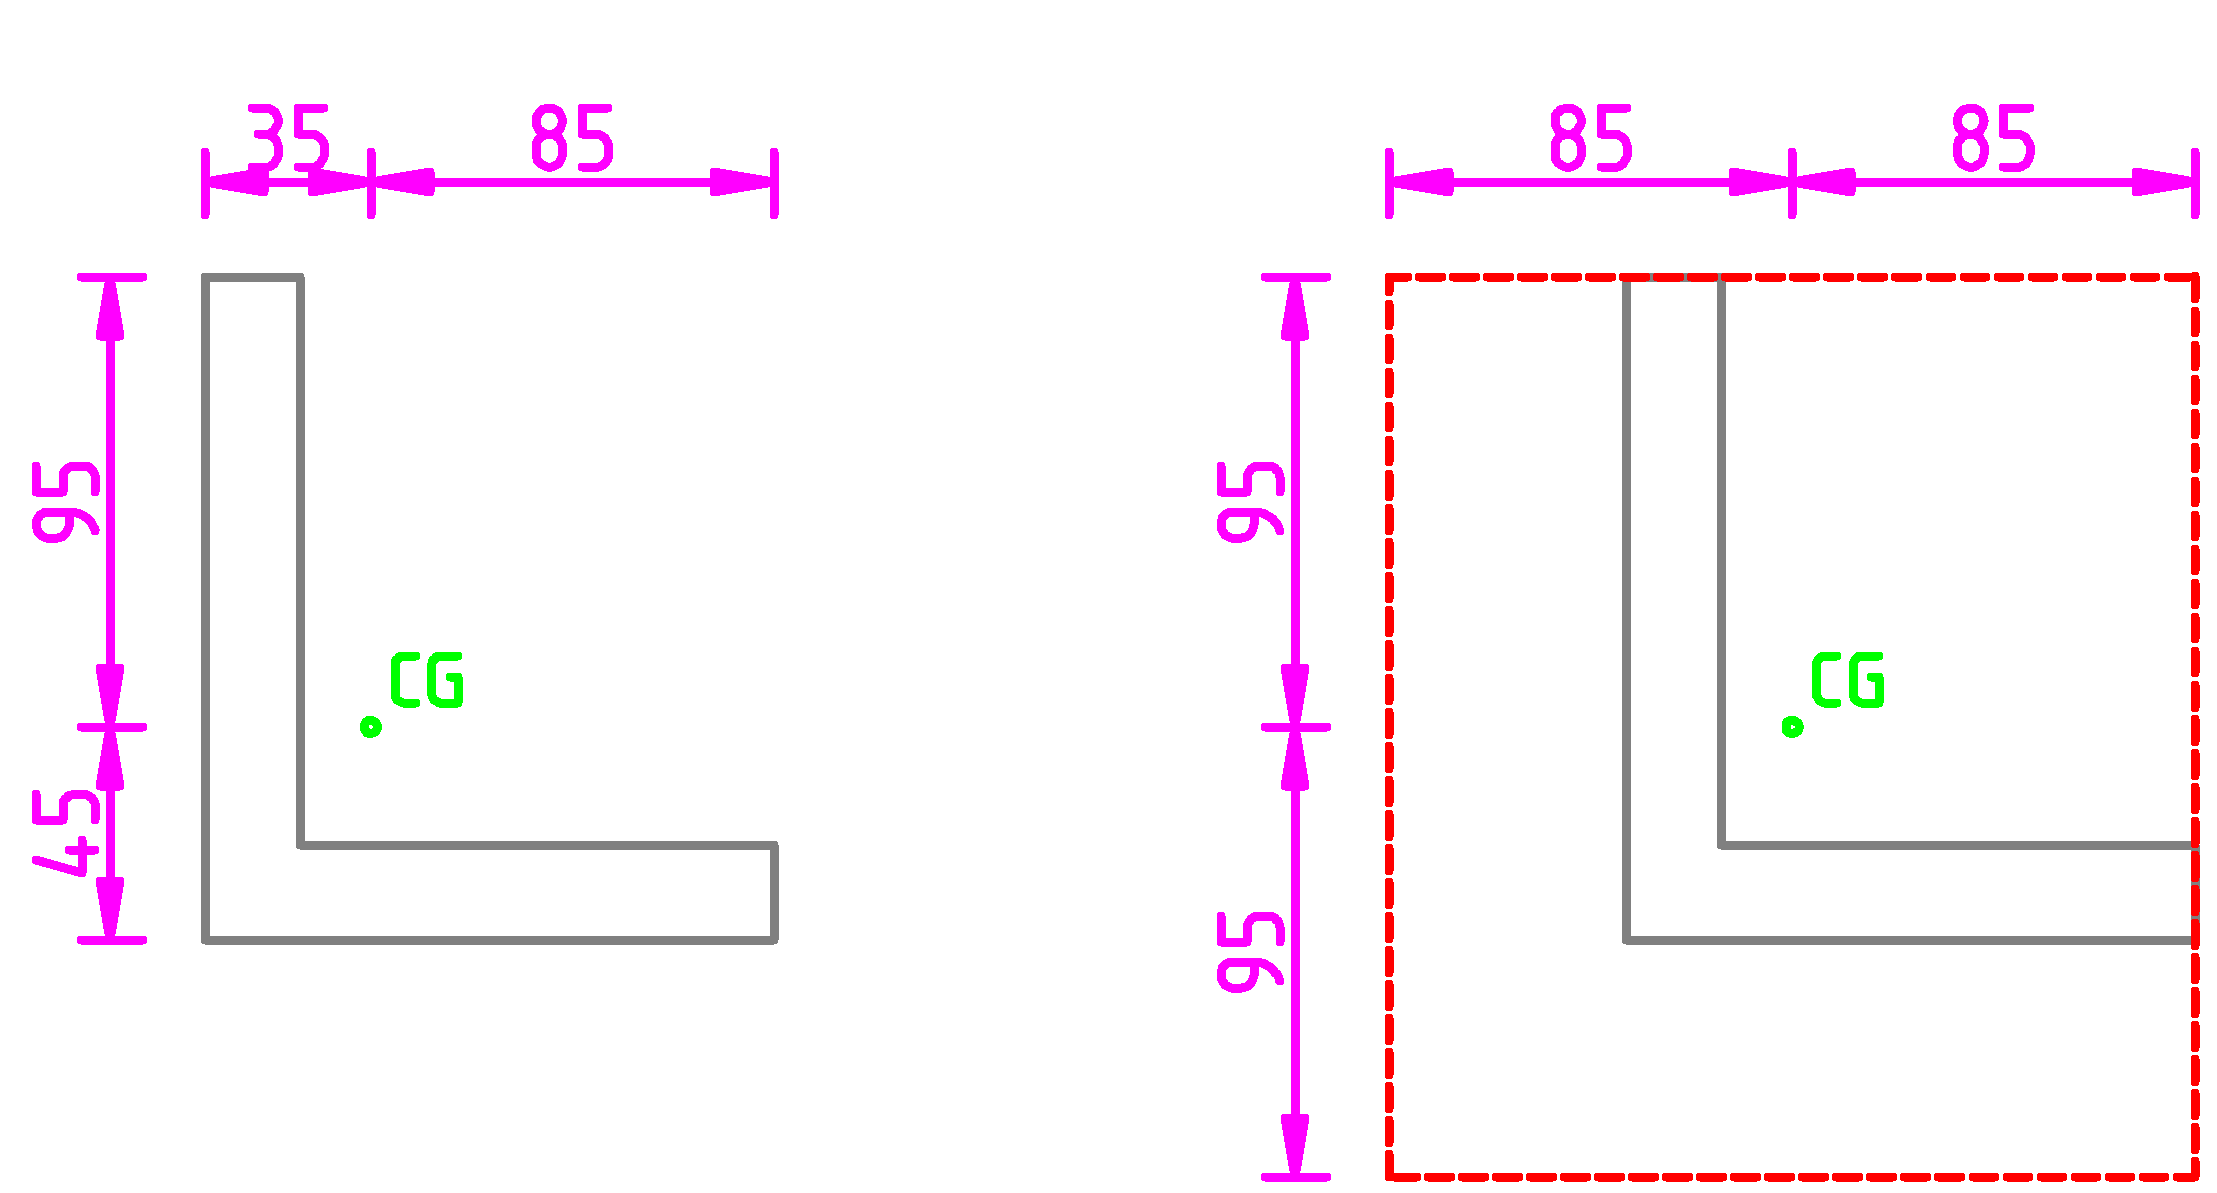
\includegraphics[width=0.8\textwidth]{Fundacoes-rasas-ou-diretas/Imagens/Exercicio-1-Sapata-conjugada-parte3.png}
	\end{center}
\end{figure}

A área necessária de sapata é:
$$A=\frac{F}{\sigma_s}=\frac{3000\;kN}{300\;kPa}=10\;m^2$$

Como $A=a\cdot b$, tem-se:
$$a=\frac{A}{b}=\frac{10\;m^2}{b}$$

Para que os momentos fletores sejam iguais nas duas direções ortogonais:
$$a-a_0=b-b_0$$
$$\frac{10}{b}-1,9=b-1,7$$

Multiplicando todos os elementos por $b$ e igualando a equação a zero, tem-se:
$$b^2+0,2\cdot b-10=0$$

As raízes (lados da sapata) são: $x_1\approx3,063\;m\approx3,1\;m$ e $x_2\approx-3,263\approx3,3\;m$.

Como o sistema é simétrico, todo o cálculo para a sapata escolhida serve para a outra sapata. Deve-se checar se a distância do CG em $x$ somada à metade de $b$ é menor que o meio do sistema, ou seja:
$$\frac{b}{2}+x_{CG}\leqslant\frac{320}{2}$$
$$\frac{310}{2}+35\leqslant160$$
$$190\leqslant160$$
\begin{figure}[H]
	\begin{center}
	\caption{Dimensões se sobrepondo na tentativa da utilização de sapata isolada.}
    	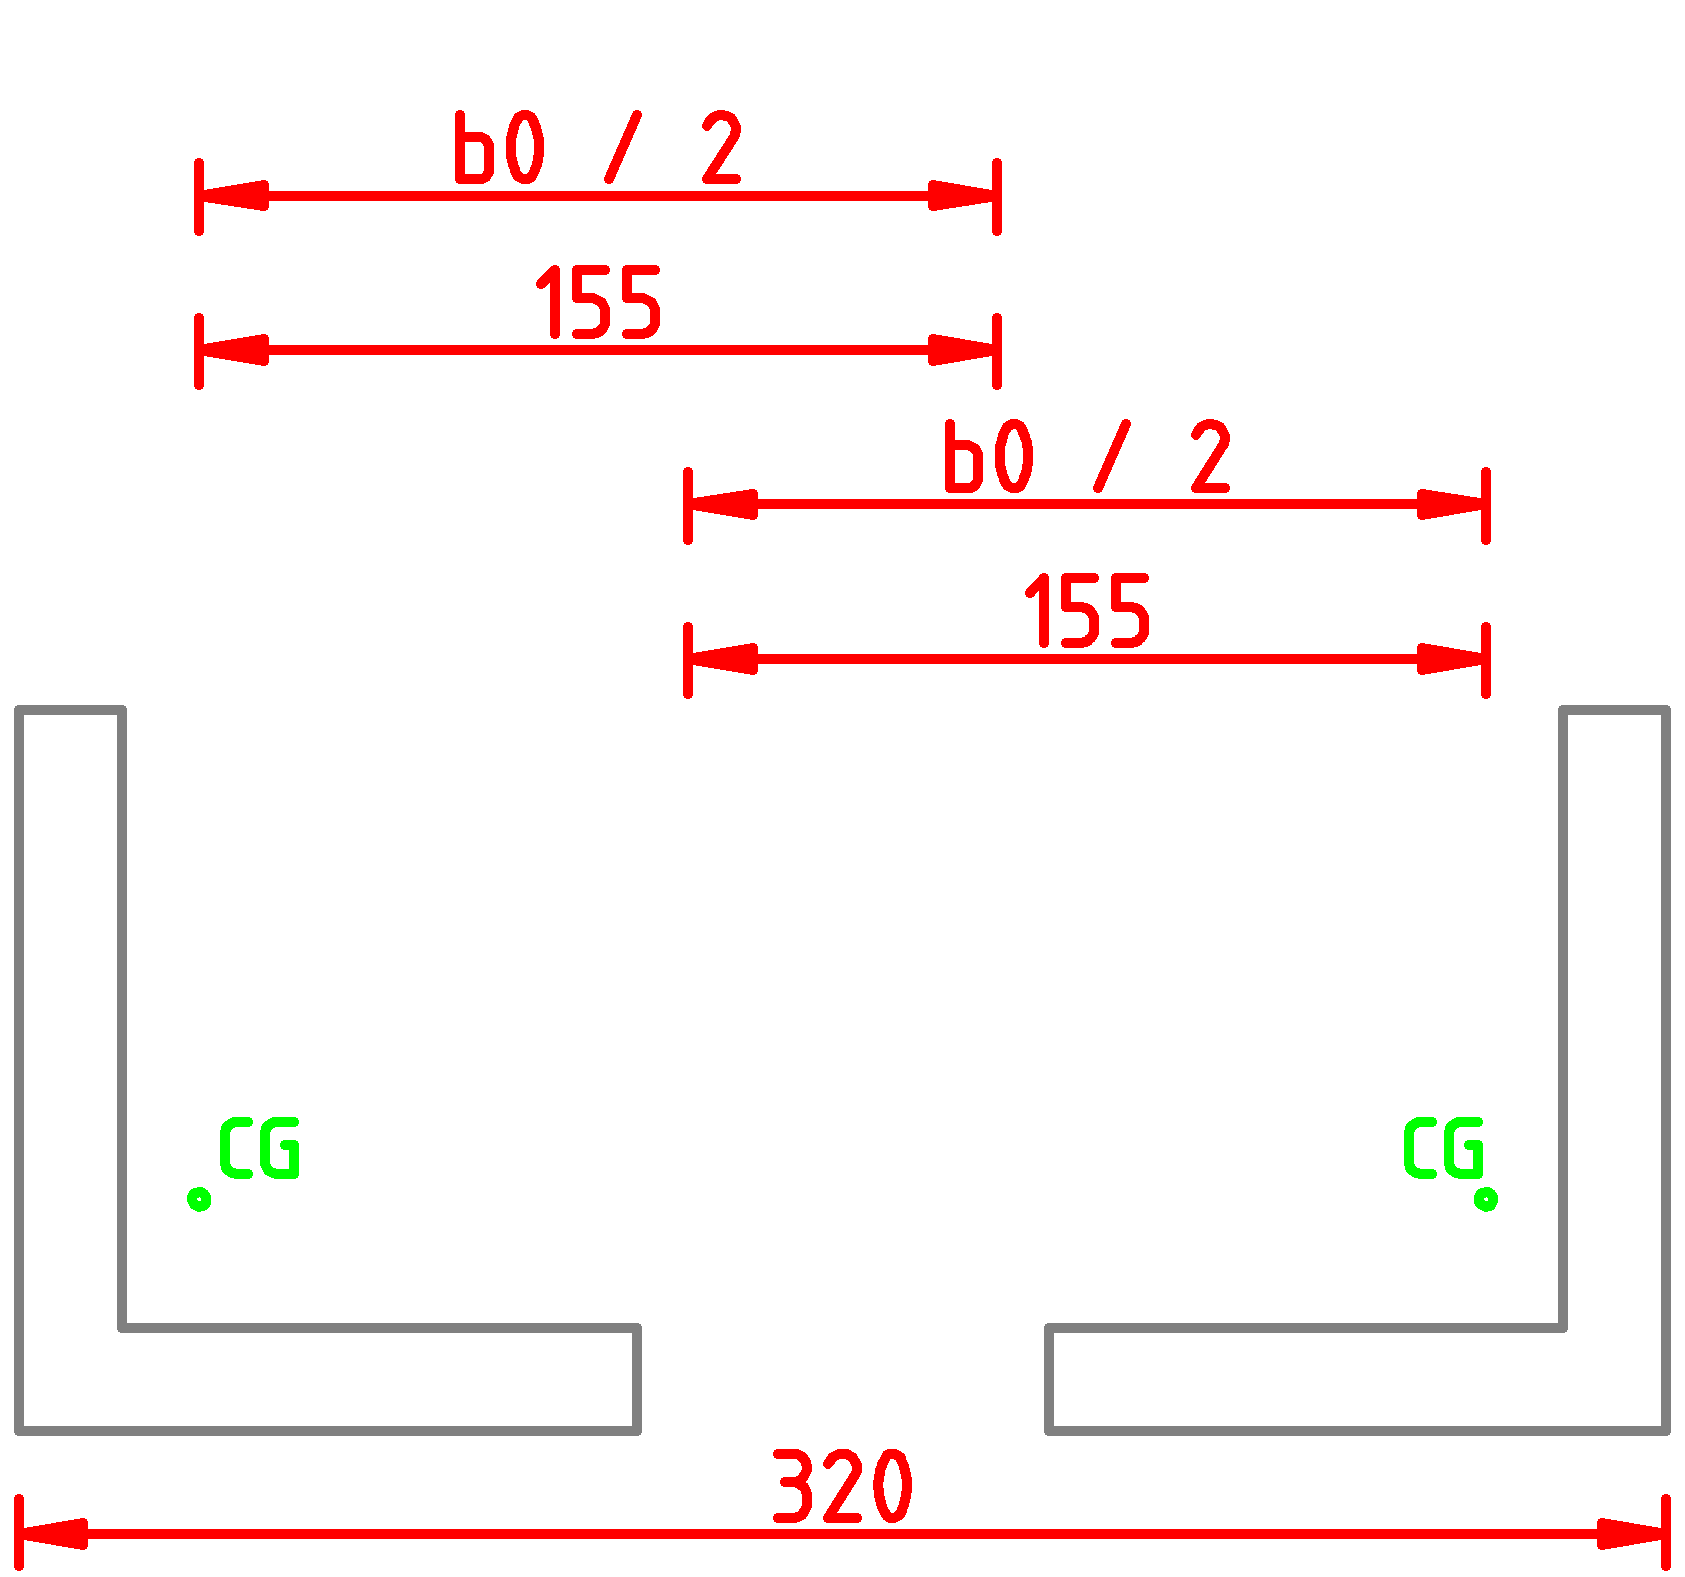
\includegraphics[width=0.6\textwidth]{Fundacoes-rasas-ou-diretas/Imagens/Exercicio-1-Sapata-conjugada-parte4.png}
	\end{center}
\end{figure}

Portanto, \textbf{não é possível fazer a solução isolada}. Neste caso, define-se a distância dos centros de carga de ambas as sapatas como $\frac{3}{5}\cdot a$, como segue:
\begin{figure}[H]
	\begin{center}
	\caption{Definição da distância entre os centros de carga dos pilares.}
    	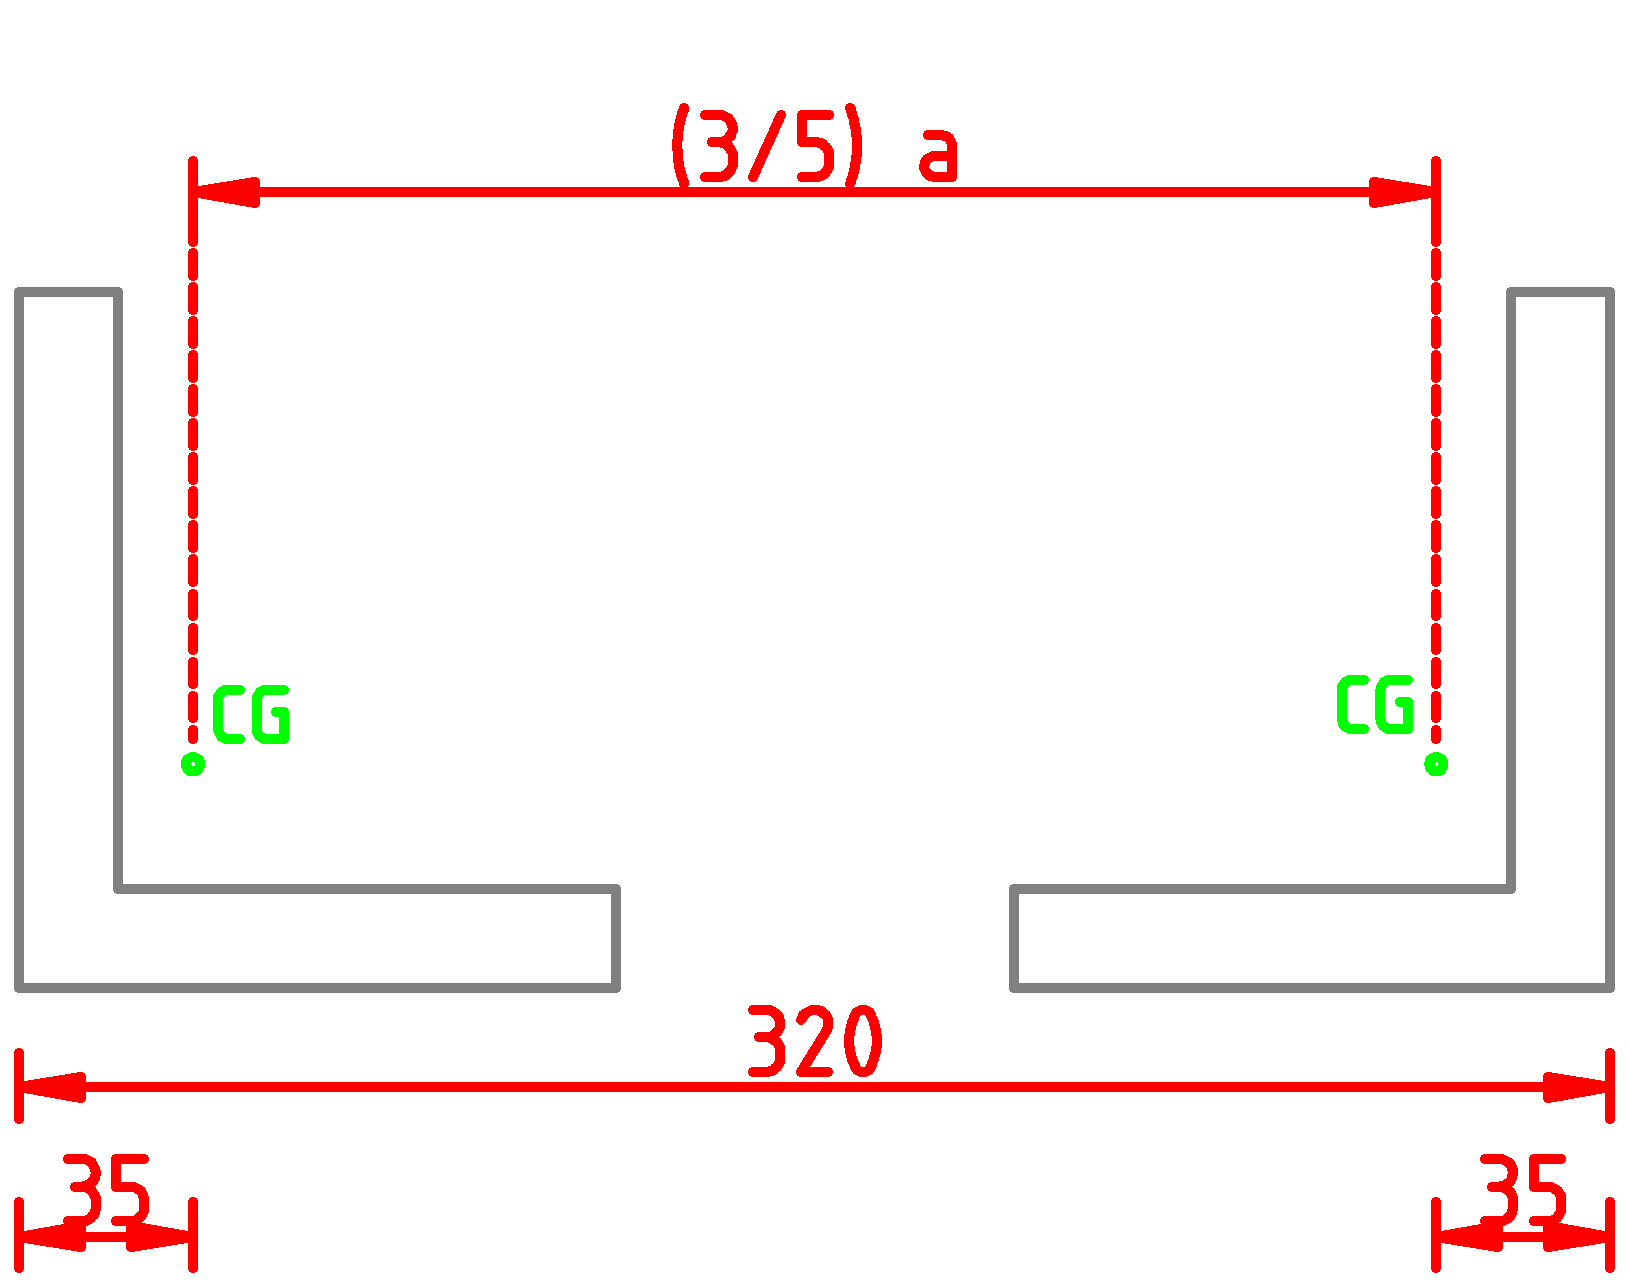
\includegraphics[width=0.6\textwidth]{Fundacoes-rasas-ou-diretas/Imagens/Exercicio-1-Sapata-conjugada-parte5.png}
	\end{center}
\end{figure}

Como a maior dimensão do pilar original está em $y$, troca-se $a$ por $b$:
$$\frac{3}{5}\cdot b=3,2\;m-(0,35\;m\cdot2)$$
$$b=\frac{2,5\;m\cdot5}{3}\approx4,17\;m\approx4,2\;m$$

A área do sistema com os dois pilares é:
$$A=\frac{P1+P2}{\sigma_s}=\frac{3000\;kN+3000\;kN}{300\;kPa}=20\;m^2$$

O lado restante da sapata conjugada é:
$$a=\frac{A}{b}=\frac{20\;m^2}{4,2\;m}\approx4,76\;m\approx4,8\;m$$

Entrando os valores de $a$ e $b$ no critério de economia:
$$2\cdot b\leqslant a\leqslant2,5\cdot b$$
$$2\cdot4,2\leqslant4,8\leqslant2,5\cdot4,2$$
$$8,4\leqslant4,8\leqslant10,5$$

Os valores encontrados de $a$ e $b$ \textbf{não} são econômicos. Portanto, inicia-se tentativas de valores para $a$ e $b$ que supram essa inequação e que forneçam a área de $20\;m^2$.

Teste com $b=2,5\;m$ e $a=8\;m$:
$$2\cdot2,5\leqslant8,0\leqslant2,5\cdot2,5$$
$$5,0\leqslant8,0\leqslant6,25$$

Teste com $b=3,2\;m$ e $a=6,4\;m$:
$$2\cdot3,2\leqslant6,4\leqslant2,5\cdot3,2$$
$$6,4\leqslant6,4\leqslant8,0$$

Portanto, as dimensões da sapata conjugada são: $a=6,4\;m$ e $b=3,2\;m$.
\begin{figure}[H]
	\begin{center}
	\caption{Sapata conjugada para o problema proposto.}
    	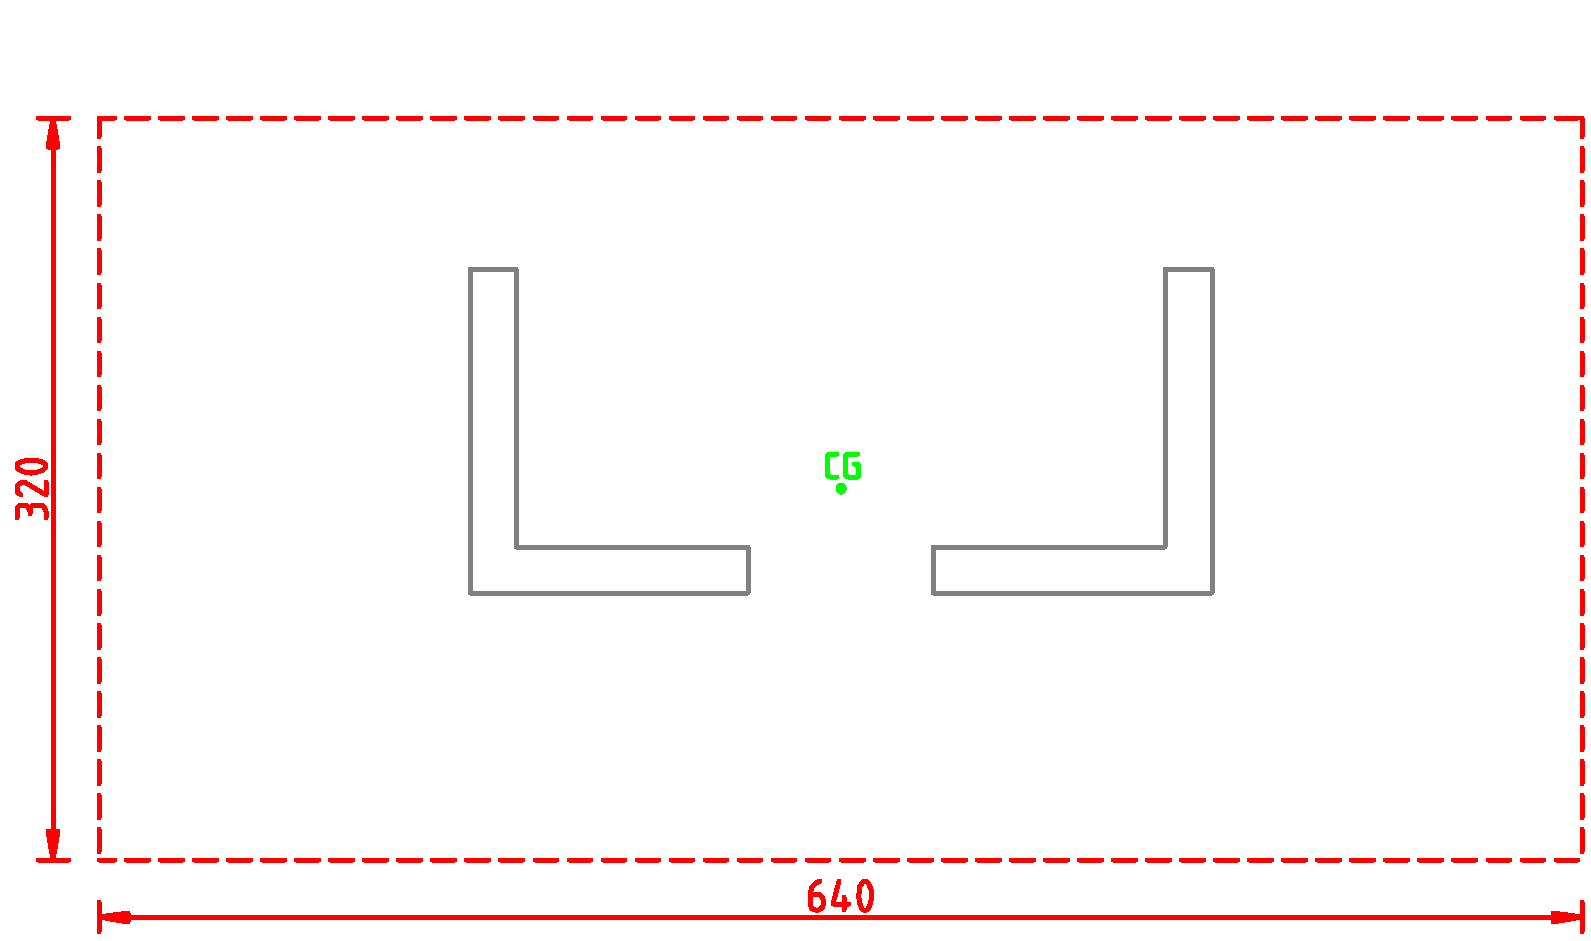
\includegraphics[width=0.7\textwidth]{Fundacoes-rasas-ou-diretas/Imagens/Exercicio-1-Sapata-conjugada-parte6.png}
	\end{center}
\end{figure}

\textbf{Exercício}: Calcular a sapata conjugada para os seguintes pilares com uma tensão admissível do solo ($\sigma_s$) de $0,3\;MPa$, $P1=3000\;kN$ e $P2=5000\;kN$:

*Inserir imagem

Calculando o centro de carga (CG) em $y$ do P2 (baseado nas subáreas):
$$y_{CG}=\frac{(150\cdot20)\cdot75+(20\cdot260)\cdot10+(20\cdot150)\cdot75}{(150\cdot20)+(20\cdot260)+(20\cdot150)}\approx44,821\;cm$$

Calculando o CG em $y$ do sistema (baseado nas cargas):
$$y_{CG}=\frac{5000\cdot44,821+3000\cdot(150+350)}{5000+3000}\approx215,513\;cm$$

O próximo passo é estimar o valor de $c$:
$$c<3\cdot y$$
$$c<3\cdot215,513\;cm=646,539\;cm$$

O intervalo de $c$ para ser escolhido de maneira arbitrária é, como na Figura X:

*Inserir figura
$$6,47\;m-(1,5\;m+3,5\;m+0,3\;m+\textbf{0,1\;m})\leqslant c < 6,47\;m$$
$$5,4\;m\leqslant c<6,47\;m$$

O valor em negrito é uma distância mínima de $10\;cm$ da face do pilar mais próximo de $b$, também arbitrário. Portanto, escolheu-se um valor de $5,5\;m$ para $c$.

O próximo passo é calcular a área necessária de sapata conjugada:
$$A=\frac{P1+P2}{\sigma_s}=\frac{3000\;kN+5000\;kN}{300\;kPa}\approx26,67m^2$$

O próximo passo é calcular o valor da parcela $(a+b)$:
$$(a+b)=\frac{2\cdot A}{c}=\frac{2\cdot26,67\;m^2}{5,5\;m}\approx9,698\;m$$

O penúltimo passo é verificar se essa parcela $(a+b)$ fornece um $b>60\;cm$:
$$b=\left[\frac{3\cdot y}{c}\cdot(a+b)\right]-(a+b)=\left[\frac{3\cdot 2,15513\;m}{5,5\;m}\cdot9,698\;m\right]-9,698\;m\approx1,703\;m\approx1,75\;m$$

Se não fornecesse um valor maior que $60\;cm$, deve-se diminuir o valor de $c$ e recalcular todos os passos seguintes. O último passo é calcular o valor de $a$:
$$a=\frac{2\cdot A}{c}-b=\frac{2\cdot26,67\;m^2}{5,5\;m}-1,703\;m\approx7,995\;m\approx8,0\;m$$